\subsection{\label{subsec:FZV1}Röntgenstrahlen}
\textbf{\textit{a) Was sind Röntgenstrahlen und wie kann man sie im elektromagnetischen
Spektrum einordnen?}}\\
$\rightarrow$Röntgenstrahlen repräsentieren elektromagnetische Wellen oder äquivalent Photonen, 
die im Wellenlängenspektrum zwischen UV-Licht und Gammastrahlen positioniert sind. 
Die exakten Grenze sind nicht präzise definiert, da sich die Spektren jeweiligen Spektren überschneiden. 
Der Wellenlängenbereich erstreckt sich ungefähr von $0,05$ bis $10\,\si{\angstrom}$ \cite{Anleitung}.
Eine Einordnung der Strahlung im gesamten elektromagnetischen Spektrum ist in Abb.~\ref{fig:spektrum}
präsentiert.
\begin{figure}[h!]
    \centering
    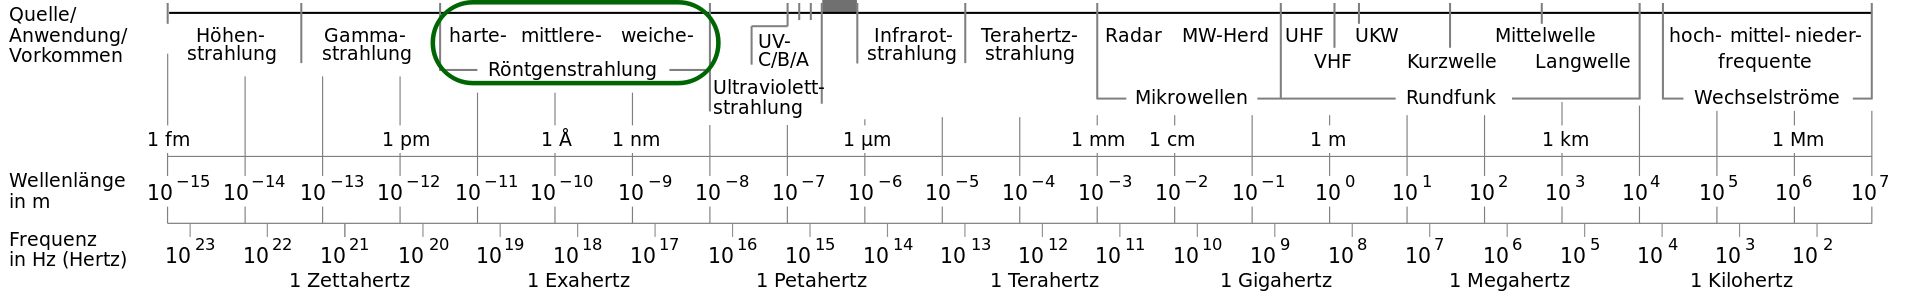
\includegraphics[width=\textwidth]{Spektrum.png}
    \caption{\label{fig:spektrum}Das gesamte elegtromagnetische Spektrum mit Angabe der Frequenz und Wellenlänge.
    Die Röntgenstrahlung (grün markiert) ist im hochenergetischen Bereich zwischen Gamma- und 
    UV-Strahlung zu finden. Die Graphik wurde Ref.~\cite{Spektrum} entnommen.}
\end{figure}  \FloatBarrier \,\\

\textbf{\textit{b) Diskutieren Sie Art und Entstehung des Emissionsspektrums einer 
Röntgenröhre.}}\\
$\rightarrow$Eine Röntgenröhre setzt sich aus einer elektronenemittierenden Kathode (aufgeheizter Wolframdraht) und einer 
matallischen Abbremskathode zusammen. Die Elektronen werden im Vakuum mittels einer angelegten Hochspannung 
($U_{\text{A}}\approx 50\,\si{kV}$)
zur Anode hin beschleunigt, in der hochenergetische Photonen durch Streuung und Elektronenübergänge entstehen \cite{Kristall}. \\
Durch Streuung der beschleunigten Elektronen am Coulombfeld der Atomkerne wird deren 
kinetische Energie in Röntgen-Photonenenergie umgewandelt, wobei ein kontinuierliches Spektrum entsteht, welches 
als Bremsspektrum bezeichnet wird. Der maximale Energieübertrag wird durch die maximal vorkommende kinetische 
Energie der Elektronen bestimmt und führt im Spektrum ($I(\lambda)$) zu einer Grenze, die invers proportional
zur Anodenspannung $U_{\text{A}}$ ist. Es gilt
\begin{align}
    E &= \frac{h\,c}{\lambda} \\
    \Rightarrow \lambda_{\text{min}} &= \frac{h\,c}{e\,U_{\text{A}}},
\end{align}
wobei $h = 6,626\cdot 10^{-34}\,\si{Js}$ das Planksche Wirkumsquantum, $c = 299\,792\,458\,\si{ms^{-1}}$ die Vakuums-Lichtgeschwindigkeit
und $e = 1,6022\cdot 10^{-19}\,\si{C}$ die Elementarladung bezeichnen. \\
Das Bremsspektrum wird von charakteristischen Linien ergänzt, die durch Photonen erzeugt werden, welche bei 
Elektronenübergängen entstehen. Die Energie der beschleunigten Elektronen reicht aus, um gebundene Elektronen 
aus ihrer Bindung und damit aus ihrer Schale zu schlagen. Die hierbei entstehenden Löcher werden von energetisch 
höher liegenden Elektronen der Bindung besetzt, wobei die Energiedifferenz als Röntgenstrahlung einer definierten 
Wellenlänge frei wird. Die Benennung der Linien berücksichtigt den spezifischen Übergang und ist 
am besten mittels eines Beispiels zu verstehen. Die $K_{\beta 2}$-Linie entsteht durch herausschlagen 
eines Elektrons in der $K$-Schale, welches von einem Elektron das zwei Schalen darüber liegt ersetzt wird  
(Abstandsnumerierung über das griechische Alphabet). Die energetische Aufspaltung aufgrund der 
Spin-Bahndrehimpuls-Kopplung wird durch die Ziffer hinter dem griechischen Buchstaben berücksichtigt,  
wobei die Zahl mit steigender Energiedifferenz zwischen den betrachteten Zuständen steigt. \\
In Abb.~\ref{fig:char} ist ein Röntgenspektrum, sowie eine schematische Darstellung der 
über die Auswahlregeln erlaubten Übergänge dargestellt.
\begin{figure}[h!]
    \centering
    \subfloat[\centering Röntgenspektrum]{{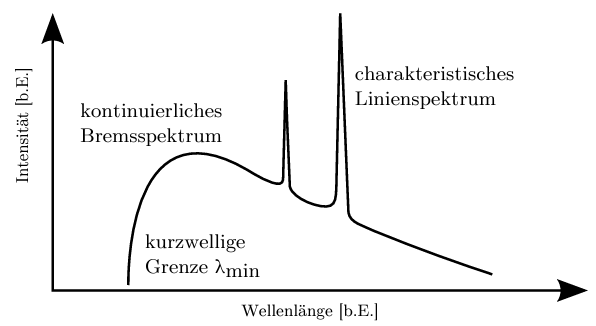
\includegraphics[width=0.65\textwidth]{RSpek.png} }}
    \qquad
    \subfloat[\centering Elektronenübergänge]{{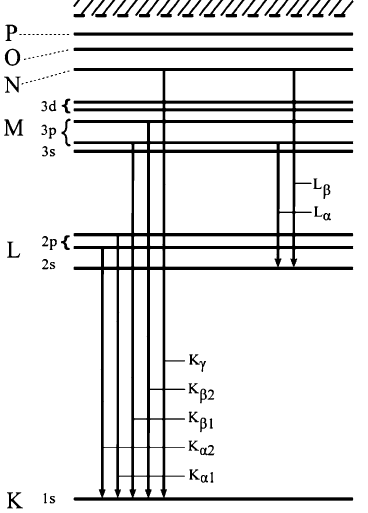
\includegraphics[width=0.25\textwidth]{Linien.png} }}
    \caption{\label{fig:char}a) Schematische Darstellung eines Röntgenspektrums, welches sich aus 
    einem kontinuierlichen Bremsspektrum und für das Anodenmaterial charakteristischen Linien zusammensetzt. 
    Wie üblich ist die Intensität der detektierten Röntgenstrahlung gegen die Wellenlänge der Strahlung aufgetragen, 
    wobei das Spektrum von einer minimalen Wellenlänge begrenzt ist. Graphik entnommen aus Ref.~[REF].\\
    b) Beispiele für erlaubte Elektronenübergänge im Energieschema inklusive Nomenklatur der darauß entstehenden Linien 
    im Spektrum. Graphik entnommen aus Ref.~\cite{Kristall}.}
\end{figure}\FloatBarrier \,\\

\textbf{\textit{c) Wie werden Röntgenstrahlen in einem Synchrotron erzeugt? Was passiert
in einem Wiggler/Undulator?}}\\
$\rightarrow$Die elektromagnetische Bremsstrahlung kann nicht nur durch das Abbremsen eines 
Elektrons durch ein Metall entstehen, sondern wird allgemein bei Beschleunigung sehr schneller 
Elektronen frei. Diese Strahlung lässt sich über die Quantenelektrodynamik erklären und 
quantifizieren, wobei die Wechselwirkung geladener Teilchen über das Photon als Austauschteilchen
verbunden ist \cite{Brems}. \\
In einem Synchrotron, einem ringförmigen Teilchenbeschleuniger, 
werden zuvor beschleunigte Elektronen mit relativistischer Energie (ungefähr 1 GeV) 
mithilfe magnetischer Strukturen abgelenkt und beschleunigt. 
Dies führt zur Erzeugung von hochenergetischer Strahlung, einschließlich Röntgenstrahlung. 
Die Elektronen werden durch Hochfrequenz-Elektromagneten beschleunigt und 
in den Speicherring injiziert. 
Dort zwingt sie das (Gradienten-)Magnetfeld auf eine Kreisbahn, 
was einer Änderung der Bewegungsrichtung, also einer Beschleunigung, entspricht. 
Dadurch werden Photonen bestimmter Energie emittiert \cite{Brems}. \\
Um die Erzeugung von Röntgenstrahlen in einem Synchrotron zu optimieren, 
kommen spezielle Vorrichtungen wie Wiggler und Undulatoren zum Einsatz. 
Bei diesen durchlaufen die Elektronen eine periodische Anordnung von abwechselnd 
orientierten Dipolmagneten. 
Dadurch beschreiben sie eine sinusförmige Bahn und emittieren Synchrotronstrahlung 
in die Ausbreitungsrichtung \cite{Wiggler}. 
Im Falle eines Wigglers werden die Elektronen stärker ausgelenkt, 
und der Abstand der umgepolten Dipolmagnete wird vergrößert. 
Dies führt zur Emission hochenergetischer Photonen, die sich nicht überlagern, 
wodurch ein breitbandiges Spektrum entsteht. 
Bei Undulatoren hingegen werden der Magnetabstand und die Auslenkung 
der Elektronen verringert, um gezielt Interferenzen der erzeugten Strahlung zu erzeugen. 
Dies führt zu einem schärferen Spektrum und höherer Brillanz \cite{Brillanz}.